\documentclass[journal,12pt,twocolumn]{IEEEtran}

\usepackage{setspace}
\usepackage{gensymb}

\singlespacing


\usepackage[cmex10]{amsmath}

\usepackage{amsthm}

\usepackage{mathrsfs}
\usepackage{txfonts}
\usepackage{stfloats}
\usepackage{bm}
\usepackage{cite}
\usepackage{cases}
\usepackage{subfig}

\usepackage{longtable}
\usepackage{multirow}

\usepackage{enumitem}
\usepackage{mathtools}
\usepackage{steinmetz}
\usepackage{tikz}
\usepackage{circuitikz}
\usepackage{verbatim}
\usepackage{tfrupee}
\usepackage[breaklinks=true]{hyperref}
\usepackage{graphicx}
\usepackage{tkz-euclide}
\usepackage{float}

\usetikzlibrary{calc,math}
\usepackage{listings}
    \usepackage{color}                                            %%
    \usepackage{array}                                            %%
    \usepackage{longtable}                                        %%
    \usepackage{calc}                                             %%
    \usepackage{multirow}                                         %%
    \usepackage{hhline}                                           %%
    \usepackage{ifthen}                                           %%
    \usepackage{lscape}     
\usepackage{multicol}
\usepackage{chngcntr}

\DeclareMathOperator*{\Res}{Res}

\renewcommand\thesection{\arabic{section}}
\renewcommand\thesubsection{\thesection.\arabic{subsection}}
\renewcommand\thesubsubsection{\thesubsection.\arabic{subsubsection}}

\renewcommand\thesectiondis{\arabic{section}}
\renewcommand\thesubsectiondis{\thesectiondis.\arabic{subsection}}
\renewcommand\thesubsubsectiondis{\thesubsectiondis.\arabic{subsubsection}}


\hyphenation{op-tical net-works semi-conduc-tor}
\def\inputGnumericTable{}                                 %%

\lstset{
%language=C,
frame=single, 
breaklines=true,
columns=fullflexible
}
\begin{document}
\newtheorem{theorem}{Theorem}[section]
\newtheorem{problem}{Problem}
\newtheorem{proposition}{Proposition}[section]
\newtheorem{lemma}{Lemma}[section]
\newtheorem{corollary}[theorem]{Corollary}
\newtheorem{example}{Example}[section]
\newtheorem{definition}[problem]{Definition}

\newcommand{\BEQA}{\begin{eqnarray}}
\newcommand{\EEQA}{\end{eqnarray}}
\newcommand{\define}{\stackrel{\triangle}{=}}
\bibliographystyle{IEEEtran}
\providecommand{\mbf}{\mathbf}
\providecommand{\pr}[1]{\ensuremath{\Pr\left(#1\right)}}
\providecommand{\qfunc}[1]{\ensuremath{Q\left(#1\right)}}
\providecommand{\sbrak}[1]{\ensuremath{{}\left[#1\right]}}
\providecommand{\lsbrak}[1]{\ensuremath{{}\left[#1\right.}}
\providecommand{\rsbrak}[1]{\ensuremath{{}\left.#1\right]}}
\providecommand{\brak}[1]{\ensuremath{\left(#1\right)}}
\providecommand{\lbrak}[1]{\ensuremath{\left(#1\right.}}
\providecommand{\rbrak}[1]{\ensuremath{\left.#1\right)}}
\providecommand{\cbrak}[1]{\ensuremath{\left\{#1\right\}}}
\providecommand{\lcbrak}[1]{\ensuremath{\left\{#1\right.}}
\providecommand{\rcbrak}[1]{\ensuremath{\left.#1\right\}}}
\theoremstyle{remark}
\newtheorem{rem}{Remark}
\newcommand{\sgn}{\mathop{\mathrm{sgn}}}
\providecommand{\abs}[1]{\vert#1\vert}
\providecommand{\res}[1]{\Res\displaylimits_{#1}} 
\providecommand{\norm}[1]{\lVert#1\rVert}
%\providecommand{\norm}[1]{\lVert#1\rVert}
\providecommand{\mtx}[1]{\mathbf{#1}}
\providecommand{\mean}[1]{E[ #1 ]}
\providecommand{\fourier}{\overset{\mathcal{F}}{ \rightleftharpoons}}
%\providecommand{\hilbert}{\overset{\mathcal{H}}{ \rightleftharpoons}}
\providecommand{\system}{\overset{\mathcal{H}}{ \longleftrightarrow}}
	%\newcommand{\solution}[2]{\textbf{Solution:}{#1}}
\newcommand{\solution}{\noindent \textbf{Solution: }}
\newcommand{\cosec}{\,\text{cosec}\,}
\providecommand{\dec}[2]{\ensuremath{\overset{#1}{\underset{#2}{\gtrless}}}}
\newcommand{\myvec}[1]{\ensuremath{\begin{pmatrix}#1\end{pmatrix}}}
\newcommand{\mydet}[1]{\ensuremath{\begin{vmatrix}#1\end{vmatrix}}}
\numberwithin{equation}{subsection}
\makeatletter
\@addtoreset{figure}{problem}
\makeatother
\let\StandardTheFigure\thefigure
\let\vec\mathbf
\renewcommand{\thefigure}{\theproblem}
\def\putbox#1#2#3{\makebox[0in][l]{\makebox[#1][l]{}\raisebox{\baselineskip}[0in][0in]{\raisebox{#2}[0in][0in]{#3}}}}
     \def\rightbox#1{\makebox[0in][r]{#1}}
     \def\centbox#1{\makebox[0in]{#1}}
     \def\topbox#1{\raisebox{-\baselineskip}[0in][0in]{#1}}
     \def\midbox#1{\raisebox{-0.5\baselineskip}[0in][0in]{#1}}
\vspace{3cm}
\title{QUIZ 1}
\author{Ananthoju Pranav Sai \\ AI20BTECH11004}
\maketitle
\newpage
\bigskip
\renewcommand{\thefigure}{\theenumi}
\renewcommand{\thetable}{\theenumi}
Download all python codes from 
\begin{lstlisting}
https://github.com/Ananthoju-Pranav-Sai/EE3900/blob/main/Quiz_1/codes
\end{lstlisting}
%
and latex-tikz codes from 
%
\begin{lstlisting}
https://github.com/Ananthoju-Pranav-Sai/EE3900/tree/main/Quiz_1/Quiz_1.tex
\end{lstlisting}
%
\section{Discrete Time Signal Processing Q 2.32}
Consider an LTI system with frequency response 
\begin{align}
    H(e^{jw}) = e^{-j\brak{\omega-\frac{\pi}{4}}}\brak{\frac{1+e^{-j2\omega}+4e^{-j4\omega}}{1+\frac{1}{2}e^{-j2\omega}}}
\end{align}
where $-\pi<\omega\leq\pi$\\
Determine the output $y[n]$ for all n if the input for all n is 
\begin{align}
    x[n] = cos\brak{\frac{\pi n}{2}}
\end{align}
\section{Solution}
Given,
\begin{align}
    H(e^{j\omega}) &= e^{\brak{\frac{j\pi}{4}}}e^{-j\omega}\brak{\frac{1+e^{-j2\omega}+4e^{-j4\omega}}{1+\frac{1}{2}e^{-j2\omega}}}\\
    x[n] &= \frac{e^{\frac{j\pi n}{2}}+e^{\frac{-j\pi n}{2}}}{2}
\end{align}
Taking fourier transform of $x[n]$
\begin{align}
    X(e^{j\omega}) = \frac{\delta(\omega-\pi/2)+\delta(\omega+\pi/2)}{2}\\
\end{align}
Now we know that
\begin{align}
    y[n] &= x[n]*h[n]
\end{align}
and by taking fourier transforms we get
\begin{align}
    Y(e^{j\omega}) &= X(e^{j\omega})H(e^{j\omega})\\
    Y(e^{j\omega}) &= \frac{H(e^{\frac{j\pi}{2}})\delta(\omega-\pi/2)+H(e^{\frac{-j\pi}{2}})\delta(\omega+\pi/2)}{2}
\end{align}
Because for any $\omega$ other than $\pm \pi/2$, $X(e^{j\omega})=0$
\begin{align}
    Y(e^{j\omega}) &= \frac{8e^{-j\pi/4}\delta(\omega-\pi/2)+8e^{j3\pi/4}\delta(\omega+\pi/2)}{2}
\end{align}
Taking inverse fourier transform of $Y(e^{j\omega})$
\begin{align}
    y[n] &= 4e^{-j\pi/4}e^{j\pi n/2}+4e^{j3\pi/4}e^{-j\pi n/2}\\
    \implies y[n] &= 4e^{j\pi/4}\brak{e^{j\pi(n-1)/2}+e^{-j\pi(n-1)/2}}\\
    \therefore y[n] &= 8e^{j\pi/4}cos\brak{\frac{\pi(n-1)}{2}}
\end{align}
\begin{figure}[!ht]
    \centering
    \resizebox{\columnwidth}{!}{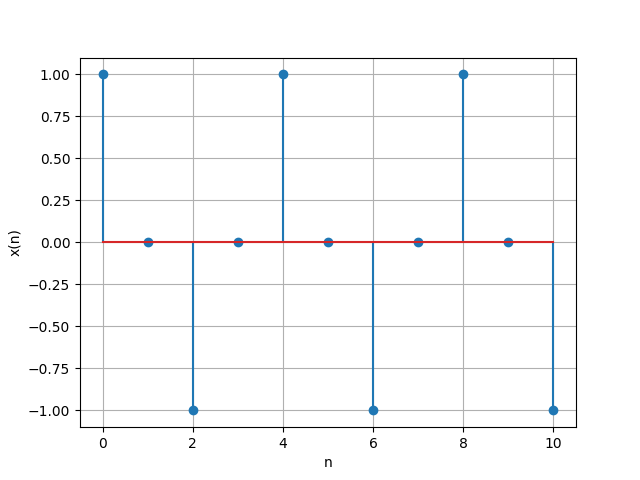
\includegraphics{input.png}}
    \caption{Input signal x[n]}
    \label{Input Signal x[n]}
\end{figure}
\begin{figure}[!ht]
    \centering
    \resizebox{\columnwidth}{!}{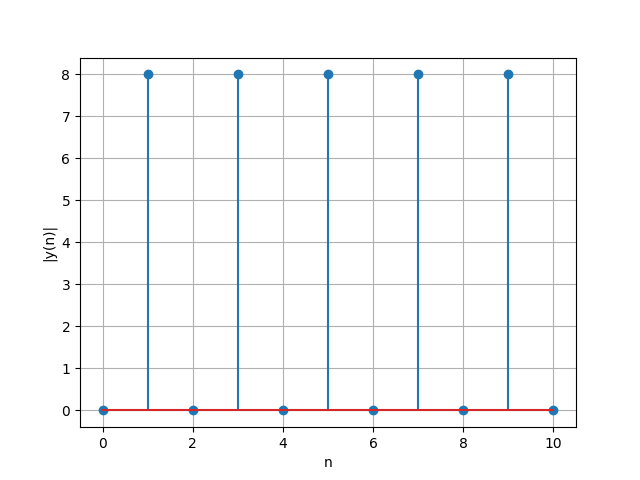
\includegraphics{output_amp.png}}
    \caption{Amplitude of y[n]}
\end{figure}
\begin{figure}[!ht]
    \centering
    \resizebox{\columnwidth}{!}{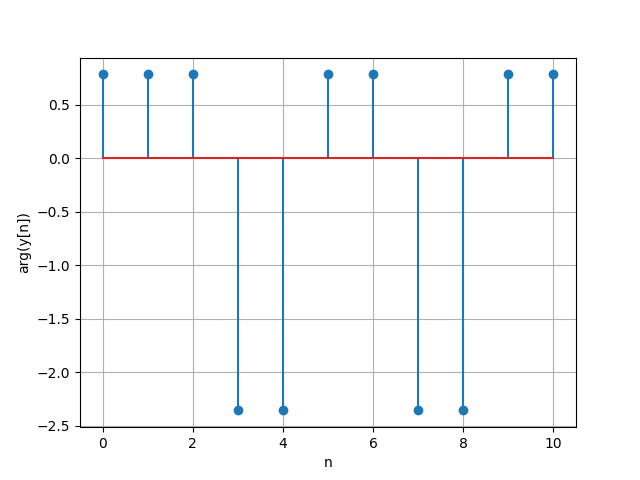
\includegraphics{output_phase.png}}
    \caption{Phase of y[n]}
\end{figure}
\end{document}